\documentclass[]{scrartcl}
\usepackage{amsmath}
\usepackage{amsfonts}
\usepackage{amssymb}
\usepackage{graphicx}

%opening
\title{Homework 7 - GNU Parallel}
\author{Alejandra Torres Manotas}
\date{}
\begin{document}

\maketitle

\section{Roots intervals definition}
The function is
\begin{equation}
	f\left(x\right)=x\cos\left(x^3-5\right).
	\label{func}
\end{equation}

Of this function I had to fine all roots in the interval $\left[0,5\right]$. 

The way to choose all intervals was choosing a step size from the part of plot in which there were more roots. In the figure (\ref{Complete}) you can see the original plot in the interval, and in the figure (\ref{Roots}) you can see the interval with more roots (the interval $\left[4.6,4.8\right]$ with five roots). Therefore the step size was $0.04$.

\begin{figure}[h]
	\centering
	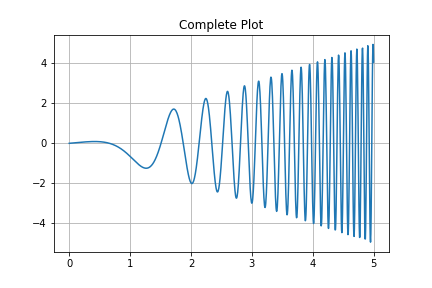
\includegraphics[scale=0.8]{Completeplot}
	\caption{Complete plot from $0$ to $5$.}
	\label{Complete}
\end{figure}

\begin{figure}[h]
	\centering
	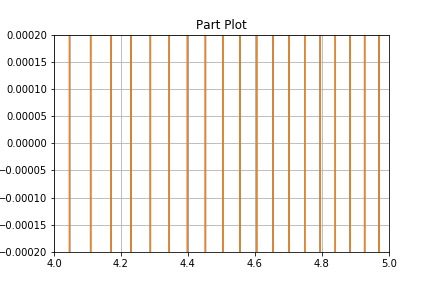
\includegraphics[scale=0.8]{roots(4-5)}
	\caption{Roots of the function (\ref{func}) from $4$ to $5$.}
	\label{Roots}
\end{figure}

\section{A serial code run in parallel}
This part of the homework is composed by two c++ codes \textit{V1.cpp} and \textit{V2.cpp}. With the first code, you can get all roots in the interval $\left[0,5\right]$ using GSL libraries. And with the second code, you can get some roots run in parallel using two shell codes \textit{script2.sh} and \textit{script2.sh} which give parameters to the main function. Thus script1 runs at the same time two different sub intervals, and script2 runs V2 code using a parallel flag of GNU Parallel and specifying how many cores will be used (two).
\end{document}
